\documentclass[xcolor=svgnames,t]{beamer} 
\usepackage[utf8]{inputenc}
\usepackage{booktabs, comment}
\usepackage{graphicx}  % Add graphicx package
\usepackage[absolute, overlay]{textpos} 
\usepackage{pgfpages}
\usepackage[font=footnotesize]{caption}
\useoutertheme{infolines} 
\usepackage{xcolor}
% \usepackage{cite}  % REMOVE this line because it conflicts with natbib
\usepackage{colortbl}
\definecolor{brownbrown}{RGB}{8, 8, 9}
\usepackage[round, sort, authoryear]{natbib}  % Use only natbib for citation management
\definecolor{brownred}{RGB}{198, 198, 198}

\setbeamercolor{title in head/foot}{bg=brownred, fg=brownbrown}
\setbeamercolor{author in head/foot}{bg=myuniversity}
\setbeamertemplate{page number in head/foot}{}

\usepackage{amsmath}
\usepackage[makeroom]{cancel}

\newtheorem{equi}{} %Creates a grey box when equi is called
\setbeamertemplate{navigation symbols}{} 
\usepackage{textpos}

\usepackage{tikz}

\usetheme{Madrid}
\definecolor{myuniversity}{RGB}{48, 67, 180}
\usecolortheme[named=myuniversity]{structure}
\usepackage{tikz}


\usepackage{colortbl} 
\newcommand{\myitem}{\item[$\circ$]}
\newcommand{\witem}{\item[\textcolor{white}{$\bullet$}]}
\DeclareMathOperator*{\argmax}{arg\,max}
\DeclareMathOperator*{\argmin}{arg\,min}
\AtBeginSection[]{
\begin{frame}
\frametitle{Content}
\tableofcontents[currentsection]
\end{frame}
}

\title[Selection on Observables]{Selection on Observables}
\subtitle{}
%\titlegraphic{\includegraphics[height=1cm]{brown-logo.png}}  % This line is commented out to remove the logo
\author[CIML ]{Causal Inference using Machine Learning\\ Master in Economics, UNT}
\institute[]{Andres Mena}
\date{Spring 2024}

\addtobeamertemplate{navigation symbols}{}{%
    \usebeamerfont{footline}%
    \usebeamercolor[fg]{footline}%
    \hspace{1em}%
    \insertframenumber/\inserttotalframenumber
}

\begin{document}
\begin{frame}
\maketitle
\end{frame}



\section{Identifications of Causal Effects under Unconfoundedness}

\begin{frame}{Confounding in Observational Studies}
\textbf{Causal Inference for Observational Studies:} 
\begin{itemize}
    \item Experimental studies are often not feasible due to ethical, practical, or financial constraints.
    \item Instead, we rely on observational data, where treatment assignment is not controlled by the researcher.
\end{itemize}

\textbf{Notation:}
\begin{itemize}
    \item Data: $\{(Y_i, D_i, X_i) : i=1,\dots,N\}$ are i.i.d. from an infinite super-population.
    \item $X_i \in \mathbb{R}^K$: vector of pre-treatment covariates.
\end{itemize}

\textbf{Key Concern: Confounding Factors}
\begin{itemize}
    \item \alert{Confounders} are variables related to both the treatment assignment and the outcome.
    \item If not properly accounted for, confounding leads to biased estimates of causal effects.
\end{itemize}
\end{frame}


\begin{frame}{Causal Graph: Potential Outcomes and Confounding}
\centering
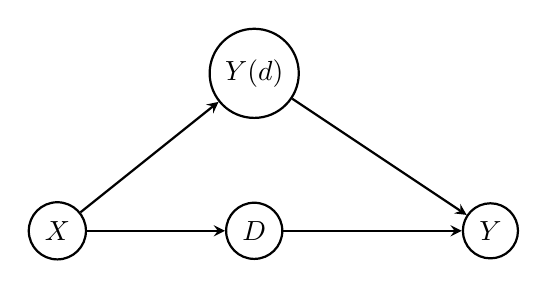
\begin{tikzpicture}[->, >=stealth, node distance=2.5cm, thick]
    % Nodes
    \node (X) [draw, circle] {$X$};
    \node (D) [draw, circle, right of=X] {$D$};
    \node (Yd) [draw, circle, above of=D, node distance=2cm] {$Y(d)$};
    \node (Y) [draw, circle, right of=D, node distance=3cm] {$Y$};
    
    % Edges
    \draw (X) -- (D);
    \draw (X) -- (Yd);
    \draw (Yd) -- (Y);
    \draw (D) -- (Y);
\end{tikzpicture}

\medskip
\begin{itemize}
    \item $X$ influences both the treatment $D$ and the potential outcomes $Y(d)$.
    \item Potential outcomes $Y(d)$ determine the realized outcome $Y$.
    \item Note: $D$ does not affect $Y(d)$ directly; $Y(d)$ is defined as the outcome \emph{if} $D$ were set to $d$.
\end{itemize}
\end{frame}


\begin{frame}{Key Assumptions}
\begin{block}{Unconfoundedness (Conditional Ignorability)}
Assumption: $(Y(1), Y(0)) \perp D \mid X$.

\end{block}
\pause
\vspace{20pt}
\begin{block}{Overlap}
Assumption: For all $x \in \mathcal{X}$, $0 < p(x) < 1$, where $p(x) = P(D=1 \mid X=x)$.

\end{block}
\end{frame}


\begin{frame}{Conditioning Removes Selection Bias}
\begin{block}{Theorem 1(Conditioning on $X$ Removes Selection Bias)}
Under Unconfoundedness and Overlap,
\[
E[Y \mid D=d, X] = E[Y(d) \mid X].
\]


\end{block}

Proof: % Leave space for handwritten proof
\end{frame}


\begin{frame}{Identification of the Average Treatment Effect (ATE)}
\begin{block}{Theorem 2 (Identification of ATE)}
\textbf{Statement:} Under Unconfoundedness and Overlap,
\[
\text{ATE} \;=\; \int_{\mathcal{X}} \bigl( E[Y \mid D=1, X=x] - E[Y \mid D=0, X=x] \bigr) \, dF_X(x).
\]


\end{block}

Proof:
\end{frame}

\section{Estimations Using Linear Regression}

\begin{frame}{Definition of ATE and ATT}
\textbf{Average Treatment Effect (ATE):}
\[
\text{ATE} = E[Y(1) - Y(0)] = \int_{\mathcal{X}} \bigl(E[Y \mid D=1, X=x] - E[Y \mid D=0, X=x]\bigr)\,dF_X(x).
\]
\pause
\textbf{Average Treatment Effect on the Treated (ATT):}
\[
\text{ATT} = E[Y(1)-Y(0) \mid D=1] = \int_{\mathcal{X}} \bigl(E[Y \mid D=1, X=x] - E[Y \mid D=0, X=x]\bigr)\,dF_{X|D=1}(x).
\]

\pause
\begin{itemize}
    \item Both ATE and ATT rely on conditional expectations $E[Y \mid D,X]$.
    \item Once we identify these conditional expectations, we integrate over the appropriate distribution of $X$.
\end{itemize}
\end{frame}

\begin{frame}{Estimating ATE and ATT by Parts (Separate Regressions)}
    \textbf{Step 1:} Estimate $E[Y|D=0,X]$ by OLS using observations with $D=0$ only. \pause
    
    \textbf{Step 2:} Estimate $E[Y|D=1,X]$ by OLS using observations with $D=1$ only. \pause
    
    \textbf{Estimate ATE:} 
    \[
    \widehat{\text{ATE}} = \frac{1}{N}\sum_{i=1}^{N} \bigl(\widehat{E}(Y|D=1,X_i) - \widehat{E}(Y|D=0,X_i)\bigr)
    \]
    \pause
    
    \textbf{Estimate ATT:}
    \[
    \widehat{\text{ATT}} = \frac{1}{N_1}\sum_{i: D_i=1} \bigl(\widehat{E}(Y|D=1,X_i) - \widehat{E}(Y|D=0,X_i)\bigr)
    \]
    where $N_1 = \sum_{i=1}^{N} 1\{D_i=1\}.$
    \end{frame}
    
    
    \begin{frame}{Estimating ATE and CATE with a Pooled Regression}
    \textbf{Pooled Model:}
    \[
    E[Y|D,X] = \alpha_1 D + \alpha_2'W D + \beta_1 + \beta_2'W,
    \]
    where $W$ includes $X$ and its transformations (centered $E[W]=0$).
    
    \pause
    
    \textbf{Interpreting Parameters:}
    \begin{itemize}
        \item ATE: $\widehat{\alpha_1}$ recovers the ATE when $W$ is centered.
        \item CATE: $\delta(X) = \alpha_1 + \alpha_2'W$ captures treatment heterogeneity.
    \end{itemize}
    
    \pause
    
    \textbf{Estimating ATT:}
    If interested in ATT, you can take the estimated conditional means from the model and average them over the treated sample distribution of $X$, analogous to the separate regressions approach:
    \[
    \widehat{\text{ATT}} = \frac{1}{N_1}\sum_{i:D_i=1} \bigl(\widehat{\alpha_1} + \widehat{\alpha_2}'W_i\bigr).
    \]
    
    \pause
    
    \textbf{Note:} In high-dimensional settings, partialling out and machine learning methods (e.g., Double Lasso) can be employed to improve flexibility and inference.
    \end{frame}
    
    \begin{frame}{Regression on the Propensity Score}
        \begin{block}{\textbf{Theorem 3: Rosenbaum \& Rubin (1983)}}
        Under unconfoundedness: 
            \[
        (Y(1), Y(0)) \perp D \mid p(X),
        \]
        where $p(X) = P(D=1 \mid X)$ is the propensity score.
        \end{block}
        \pause
        \textbf{Implication:} 
        \begin{itemize}
            \item Under unconfoundedness, conditioning on $p(X)$ (the propensity score) suffices to remove confounding.
            \item This allows for more parsimonious models by reducing the dimensionality of $X$.
        \end{itemize}
        
        \pause
        
       
    \end{frame}
        
     \begin{frame}
        \textbf{Steps for Propensity Score Regression:}
        \begin{enumerate}
            \item \textit{Estimate} $p(X)$ using a flexible binary regression model (e.g., logistic regression or machine learning methods).
            \pause
            
            \item \textit{Run regressions} to estimate $E(Y \mid D=d, p(X))$ using the estimated propensity scores $\widehat{p}(X)$.
            \pause
            \item \textit{Compute:}
            \[
            \widehat{\delta}(x_i) = \widehat{E}(Y \mid D=1, p=\widehat{p}(X_i)) - \widehat{E}(Y \mid D=0, p=\widehat{p}(X_i)).
            \]
            \pause
            \item \textit{Take the sample average of $\widehat{\delta}(x_i)$ to estimate ATE or ATT.}
        \end{enumerate}
     \end{frame}   
        
        \begin{frame}{Propensity Score Blocking}
        \textbf{Alternative Approach: Propensity Score Blocking}
        \begin{itemize}
            \item Divide the range of $\widehat{p}(X)$ into blocks or strata (e.g., deciles).
            \pause
            \item Within each block, assume $E(Y \mid D, p(X))$ is approximately constant.
            \pause
            \item Estimate $E(Y \mid D=d, p(X))$ within each block as the average outcome for treated ($D=1$) and control ($D=0$) units.
            \pause
            \item Aggregate across blocks to compute:
            \[
            \widehat{\text{ATE}} = \frac{1}{N} \sum_{i=1}^N \bigl(\widehat{E}(Y \mid D=1, p=\widehat{p}(X_i)) - \widehat{E}(Y \mid D=0, p=\widehat{p}(X_i))\bigr).
            \]
        \end{itemize}
        
        \pause
        
        \textbf{Pros:}
        \begin{itemize}
            \item Nonparametric approach that avoids imposing a functional form on $E(Y \mid D, p(X))$.
        \end{itemize}
        
        \textbf{Cons:}
        \begin{itemize}
            \item Requires sufficient sample size within each block to ensure reliable estimates.
            \item Sensitivity to the choice of the number and width of blocks.
        \end{itemize}
        \end{frame}
        




\section{Inverse Probability Weighting}


\begin{frame}{Proving Identification of \(E[Y(0)]\) and \(E[Y(1)]\) Using IPW}
    \begin{block}{\textbf{Theorem 4 (Horvitz-Thompson: Propensity Score Reweighting Removes Bias)}}
        \[
        E \left[ \frac{Y \cdot 1(D=d)}{P(D=d|X)} \mid X \right] = E[Y(d) \mid X]
        \]
        \end{block}

\textbf{Proof Outline:}

\end{frame}


\begin{frame}{Estimating ATE and ATT Using IPW}
\textbf{ATE Estimation Using the Horvitz-Thompson Formula:}
\[
\widehat{\text{ATE}}_{\text{IPW}} = \frac{1}{N} \sum_{i=1}^N \left[
\frac{D_i Y_i}{\widehat{p}(X_i)} - \frac{(1-D_i) Y_i}{1-\widehat{p}(X_i)}
\right].
\]
\pause
\textbf{Normalized Propensity Score Weighting (Recommended):}
\begin{itemize}
    \item Adjust weights to sum to 1 within treated and control groups for improved stability.
\end{itemize}

\pause

\textbf{ATT Estimation Using IPW:}
\[
\widehat{\text{ATT}}_{\text{IPW}} = \frac{1}{N_t} \sum_{i:D_i=1} Y_i - \frac{1}{N_c} \sum_{i:D_i=0} \frac{\widehat{P(D=0)}}{\widehat{P(D=1)}} \frac{Y_i}{1-\widehat{p}(X_i)}.
\]

\pause

\textbf{Role of Propensity Score Weighting:}
\begin{itemize}
    \item Equalizes the distribution of \(X\) across treatment and control groups.
    \item For ATE: \(X \mid D=1\) weighted by \(P(D=1)/p(X)\) matches the marginal distribution of \(X\).
    \item For ATT: \(X \mid D=0\) weighted by \(\frac{P(D=0)p(X)}{P(D=1)(1-p(X))}\) matches \(X \mid D=1\).
\end{itemize}
\end{frame}


\section{Doubly Robust Estimation}

\begin{frame}{Doubly Robust Methods}
    \textbf{Setup:}
    \begin{itemize}
        \item Let \(E(Y \mid D=d, X=x) = E(Y(d) \mid X=x) = \mu_d(x; \beta)\), the outcome regression model.
        \item Let \(P(D=1 \mid X=x) = p(x; \gamma)\), the propensity score model.
    \end{itemize}
    
    \pause
    
    \textbf{Moment Condition for \(\theta_{\text{ATE}}\):}
    \scriptsize
    \[
    \theta_{\text{ATE}} = E \left[
    \mu_1(X; \beta) - \mu_0(X; \beta)
    + \frac{D(Y - \mu_1(X; \beta))}{p(X; \gamma)}
    - \frac{(1-D)(Y - \mu_0(X; \beta))}{1-p(X; \gamma)}
    \right].
    \]
    \normalsize
    
    \pause
    
    \textbf{Doubly Robust (DR) Estimator for \(\theta_{\text{ATE}}\):}
    \scriptsize
    \[
    \widehat{\theta}_{\text{DR, ATE}} = \frac{1}{N} \sum_{i=1}^N \left[
    \mu_1(X_i; \widehat{\beta}) - \mu_0(X_i; \widehat{\beta})
    + \frac{D_i(Y_i - \mu_1(X_i; \widehat{\beta}))}{\widehat{p}(X_i; \widehat{\gamma})}
    - \frac{(1-D_i)(Y_i - \mu_0(X_i; \widehat{\beta}))}{1-\widehat{p}(X_i; \widehat{\gamma})}
    \right].
    \]
    \normalsize
    
    \pause
    
    \textbf{Key Properties:}
    \begin{itemize}
        \item \textbf{Doubly Robust:} The estimator is consistent if either:
        \begin{itemize}
            \item The outcome regression model \(\mu_d(X; \beta)\) is correctly specified, OR
            \item The propensity score model \(p(X; \gamma)\) is correctly specified.
        \end{itemize}
        \pause
        \item \textbf{Efficiency:} If both models are correctly specified, the estimator is more efficient than using either model alone.
       
    \end{itemize}
    \end{frame}
    
    


\section{Neyman Orthogonality}

\begin{frame}{Neyman Orthogonality }
    \textbf{Motivation:} In modern econometrics, we often estimate causal parameters \(\theta\) while also estimating high-dimensional nuisance functions \(\beta\) and/or \(\gamma\). Examples include:
    \begin{itemize}
        \item Outcome regression functions \(\mu_d(X; \beta)\)
        \item Propensity scores \(p(X; \gamma)\)
    \end{itemize}
    
    \pause
    
    \textbf{Problem:} Naive estimators are sensitive to estimation errors in these nuisance parameters. If \(\widehat{\beta}\) or \(\widehat{\gamma}\) converge slowly, such errors can cause large biases in the causal parameter estimates.
    
    \pause
    
    \textbf{Neyman Orthogonality:} A property of a moment equation (or estimator) that makes it \emph{insensitive} to small perturbations in the nuisance parameter estimates. Formally, the first-order derivative of the moment condition with respect to the nuisance parameters at the true value is zero. This ensures that small estimation errors in \(\beta\) or \(\gamma\) do not induce first-order bias in the estimator of \(\theta\).
    \end{frame}
    
    
    \begin{frame}{Naive estimatior}
    \textbf{Comparison: Regression-based Estimator for ATE}
    
    Consider a regression-based ATE estimator:
    \[
    \widehat{\theta} = \frac{1}{N}\sum_{i=1}^N [\mu_1(X_i; \widehat{\beta}) - \mu_0(X_i; \widehat{\beta})] = \frac{1}{N} \sum^N_{i=1} \Delta \mu (X_i, \hat{\beta}).
    \]
    
    \pause
    
    \textbf{Taylor Expansion:} Let \(\theta_0\) be the true ATE and \(\beta_0\) the true parameter. Using a Taylor expansion around \(\beta_0\):
    \[
    \sqrt{N}(\widehat{\theta} - \theta_0) = \frac{1}{\sqrt{N}}\sum_{i=1}^N m_{1i}(\beta_0) 
    + G_{\beta} \cdot \sqrt{N}(\widehat{\beta}-\beta_0) + o_p(1),
    \]
    \pause
    \scriptsize
    where: \\
    - \(G_{\beta}\) is the \textbf{derivative (gradient)} of the estimator's moment condition with respect to \(\beta\) at \(\beta_0\).\\
    \pause
    - $m_{1i}(\beta_0)=\Delta \mu (X_i, \hat{\beta}) - E[\Delta \mu (X_i, \hat{\beta})] $ 
    
    \pause
    
    \textbf{Consequence:}
    If \(\widehat{\beta}-\beta_0\) converges more slowly than \(N^{-1/2}\), the term \(G_{\beta} \cdot \sqrt{N}(\widehat{\beta}-\beta_0)\) introduces a first-order bias. Hence, the accuracy of \(\widehat{\theta}\) critically depends on the rate at which \(\widehat{\beta}\) converges.
    
    \end{frame}
    
    
    \begin{frame}{Neyman Orthogonality and Double Robustness }
        \textbf{Double Robust (DR) Estimator for ATE:}
        {\scriptsize
        \[
        \widehat{\theta}_{\text{DR}} = \frac{1}{N}\sum_{i=1}^N \left[
        (\mu_1(X_i;\widehat{\beta}) - \mu_0(X_i;\widehat{\beta}))
        + \frac{D_i(Y_i - \mu_1(X_i;\widehat{\beta}))}{\widehat{p}(X_i;\widehat{\gamma})}
        - \frac{(1-D_i)(Y_i - \mu_0(X_i;\widehat{\beta}))}{1-\widehat{p}(X_i;\widehat{\gamma})}
        \right].
        \]
        }
        \pause
        
        \textbf{Taylor Expansion of the DR Estimator:} Let \(\psi(X_i; \beta, \gamma)\) represent the influence function in the above bracketed term. Expanding around \((\beta_0,\gamma_0)\):
        {\scriptsize
        \[
        \widehat{\theta}_{\text{DR}} - \theta_0 
        = \frac{1}{N}\sum_{i=1}^N [\psi(X_i; \beta_0,\gamma_0) - E\{\psi(X;\beta_0,\gamma_0)\}]
        + \frac{1}{N}\sum_{i=1}^N \left(\frac{\partial \psi}{\partial \beta}, \frac{\partial \psi}{\partial \gamma}\right)\bigg|_{(\beta_0,\gamma_0)} 
        (\widehat{\beta}-\beta_0, \widehat{\gamma}-\gamma_0)' + o_p(1).
        \]
        }
        \pause
        \scriptsize
        \textbf{Neyman Orthogonality:} For the DR estimator, the partial derivatives \(\frac{\partial \psi}{\partial \beta}\) and \(\frac{\partial \psi}{\partial \gamma}\) at \((\beta_0,\gamma_0)\) are zero. Hence:
        \[
        G_{\beta} = \frac{\partial E[\psi]}{\partial \beta}\bigg|_{\beta_0,\gamma_0} = 0, \quad
        G_{\gamma} = \frac{\partial E[\psi]}{\partial \gamma}\bigg|_{\beta_0,\gamma_0} = 0.
        \]
        
        \pause
        
        
        \textbf{Implications:}
        \begin{itemize}
            \item With \(G_{\beta}=G_{\gamma}=0\), the leading bias terms vanish.
            \item The DR estimator is robust to first-order estimation errors in \(\beta\) and \(\gamma\).
            \item If either the outcome model or the propensity score model is correctly specified, the DR estimator remains consistent, making it highly valuable in high-dimensional or complex modeling scenarios.
        \end{itemize}
        \end{frame}
          
    
   
    


\end{document}


































 


